\begin{center}
	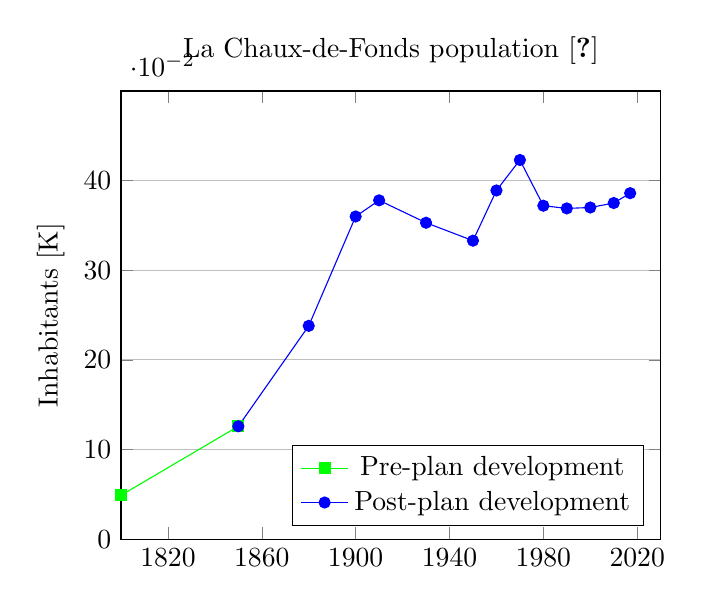
\begin{tikzpicture}
		\begin{axis}[
				title={La Chaux-de-Fonds population  \cite{Wikimedia:LaChauxDeFonds}},
				style={/pgf/number format/1000 sep=},
				ylabel={Inhabitants [K]},
				xmin=1800, xmax=2030,
				ymin=0, ymax=0.05,
				xtick={1820,1860,1900,1940,1980,2020},
				ytick={0,0.01,0.02,0.03,0.04},
				yticklabels={0,10,20,30,40},
				legend pos=south east,
				ymajorgrids=true
			]	
			\addplot[color=green,mark=square*] coordinates {
				(1750,0.0023)(1800,0.0049)(1850,0.0126)
			};
			\addplot[color=blue,mark=otimes*] coordinates {
				(1850,0.0126)(1880,0.0238)(1900,0.0360)(1910,0.0378)(1930,0.0353)(1950,0.0333)(1960,0.0389)(1970,0.0423)(1980,0.0372)(1990,0.0369)(2000,0.0370)(2010,0.0375)(2017,0.0386)
			};
			\legend{Pre-plan development,Post-plan development}	
		\end{axis}
	\end{tikzpicture}
\end{center}
